\documentclass[12pt,a4paper]{article}
\usepackage[utf8]{inputenc}
\usepackage{amsmath}
\usepackage{amsfonts}
\usepackage{amssymb}
\usepackage{graphicx}
\usepackage{cancel}
\usepackage{geometry}
\renewcommand*\thesection{\alph{section})}
\usepackage[ngerman]{babel}
\geometry{a4paper, top=20mm, left=15mm, right=15mm, bottom=20mm}
\author{Marius Ketterer}
\title{Versuch 2 - Digitales Regelungssystem - Lösung}
\begin{document}
		\maketitle
	\tableofcontents

	
	\newpage
	\section{Berechnen Sie die z-Übertragungsfunktion der Strecke inkl. Halteglied}
	
	\subsection{Übertragunsfunktion der Strecke}
	\begin{equation}
	G_s(s) = \frac{K_s}{(1+T_ss)T_is} \text{mit} K_s = 3;T_s = 1;T_i = 3
	\end{equation}
	
	\begin{equation}
	G_s(s) = \frac{\cancel{3}}{(1+s)\cancel{3}s}
	\end{equation}
	\subsection{z-Transformation mit Halteglied}
	\begin{equation}
	G_s(z) = (1-z^{-1}) 
	\mathcal{Z}
	\left\{
		\frac{G_s(s)}{s}
	\right\} =
	(1-z^{-1}) 
	\mathcal{Z}
	\left\{
		\frac{1}{s^2(1+s)}
	\right\} 
	\end{equation}
	Transformieren mit Hilfe der Korrespondenzentabelle(Nr.13)
	
	\begin{equation}
	G_s(z) = \cancel{(1-z^{-1})} 
	\frac{\left[(T_A-1+e^{-T_A})+(1-e^{-T_A}-aT_Ae^{-T_A})z^{-1}\right]z^{-1}}
	{(1-z^{-1})^{\cancel{2}}(1-e^{-T_A}z^{-1})}
	\end{equation}
	Nun wird die Abtastzeit $T_A=0,2$ eingesetzt und ausmultipliziert
	\begin{equation}
	G_s(z)= \frac
	{0,0175z^{-2}+0,019z^{-1}}
	{0,819z^{-2}-1,819z^{-1}+1}
	\end{equation}
	\section{Berechnen der Führungsübertragungsfunktion und der Führungssprungantwort}
	\begin{equation}
	G_R(z)= K_R =5
	\end{equation}
	\begin{equation}
	G_w(z)=\frac{G_R(z)\cdot G_s(z)}{1+G_R(z)\cdot G_s(z)} = 
	\frac{\frac{5Z(z)}{N(z)}}{1+\frac{5Z(z)}{N(z)}} = \frac{5Z(z)}{N(z)+Z(z)}
	\end{equation}
	Daraus ergibt sich wenn man Zähler und Nenner wieder einsetzt
	\begin{equation}
	G_w(z)= \frac
	{0,0875z^{-2}+0,095z^{-1}}
	{0,9065z^{-2}-1,724z^{-1}+1}
	\end{equation}
	
	Berechnen der ersten 6 Werte der Führungssprungantwort\\
%	\begin{table}
%		\centering
%		\caption{Die ersten 6 Werte der Führungssprungantwort}
		\begin{tabular}{c|c|c}
			n & $w_n$&$x_n$ \\ \hline
			0&1&0  \\ \hline
			1&1&0,095  \\ \hline
			2&1&0,3463  \\ \hline	
			3&1&0,6934  \\ \hline
			4&1&1,064  \\ \hline
			5&1&1,388  \\ 
		\end{tabular}
%	\end{table}
\newpage
\section{Simulationsergebnisse Führungsübertragungsfunktion}
\begin{figure}[h!]
	\centering
	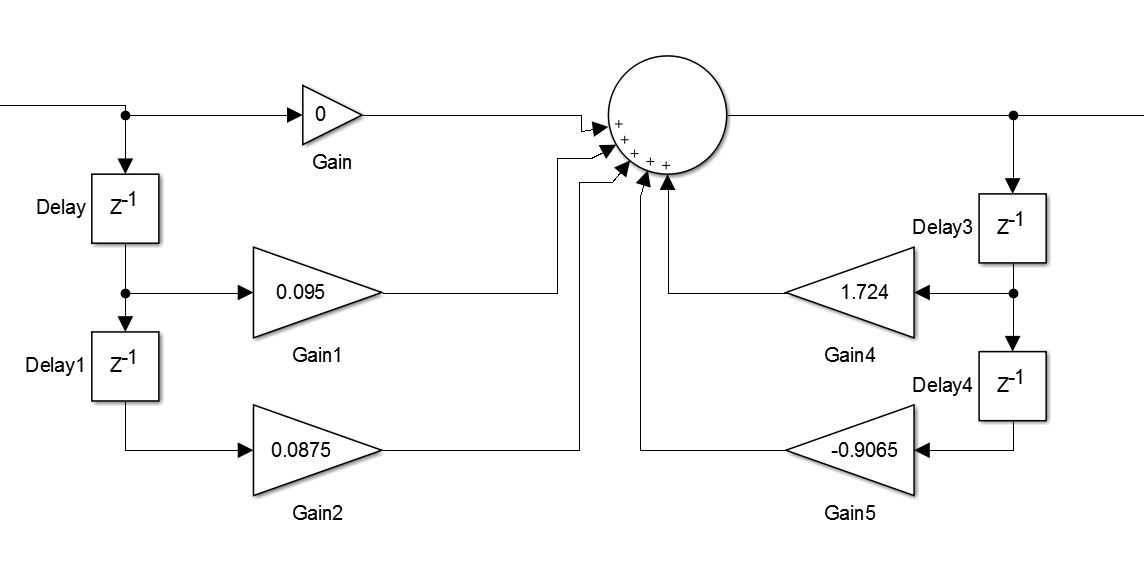
\includegraphics[width=0.7\linewidth]{D:/Git/RT2_PR_Abgaben/RT2_Abgaben_marius/marius/V2/Gwz}
	\caption{Struckturplan von $G_w(z)$}
	\label{fig:gwz}
\end{figure}
\begin{figure}[h!]
\centering
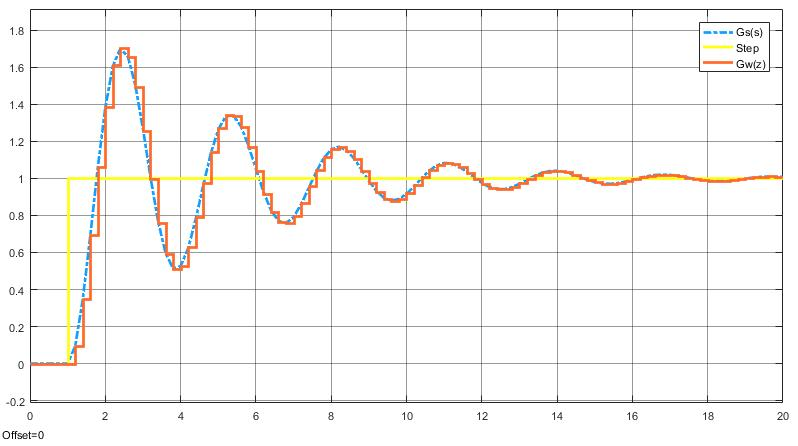
\includegraphics[width=1\linewidth]{D:/Git/RT2_PR_Abgaben/RT2_Abgaben_marius/marius/V2/Fuehrungsuebertragungsfkt}
\caption{Führungssprungantwort}
\label{fig:fuehrungsuebertragungsfkt}
\end{figure}
\newpage
\section{Berechnen der bleibenden Regelabweichung}
\begin{equation}
w(s)= \frac{w_0}{s} = \frac{1}{s} \text{mit} w_0 = 1 \text{(Einheitssprung)}
\end{equation}
Aus dem Blockschaltbild ergibt sich folgender Zusammenhang:
\begin{equation}
x(s) = w(s)*G_w(s) = \frac{1}{s}\cdot \frac{5}{s^2+s+5}
\end{equation}
Transformation in den Zeitbereich
\begin{equation}
x(t) = 5\left[
\frac{1}{5}-
\frac
	{e^{-\frac{t}{2}(\sin(\frac{\sqrt{19}t}{2})+\sqrt{19}\cos(\frac{\sqrt{19}t}{2}))}}
{5\sqrt{19}}
\right]
\end{equation}
\begin{equation}
\lim t\rightarrow \infty:
\end{equation}
\begin{equation}
x(t) = 5\cdot \left( \frac{1}{5}-0\right) =1
\end{equation}
Bleibende Regelabweichung $x_b$:
\begin{equation}\label{key}
x_b = w_0 -x(t\rightarrow \infty) = 1-1=0
\end{equation}



\section{Störübertragungsfunktion und Störsprungantwort brechnen}

Durch das Blockschaltbild kann man folgende Gleichung aufstellen:
\begin{equation}
x(z)=v(z)-x(z)G_RG_S
\end{equation}
Löst man diese Gleichung nach $x(z)$ erhält man dies:
\begin{equation}
x(z)= \frac{v(z)}{1+G_RG_S}
\end{equation}
Wodurch sich die Störübertragungsfunktion
\begin{equation}
G_v(z) = \frac{x(z)}{v(z)} = \frac{1}{1+G_RG_S} = \frac{0,819z^{-2}-1,819z^{-1}+1}{0,9065z^{-2}-1,174z^{-1}+1}
\end{equation}

	Berechnen der ersten 6 Werte der Störungssprungantwort\\
		\begin{tabular}{c|c|c}
			n & $v_n$&$x_n$ \\ \hline
			0&1&1  \\ \hline
			1&1&0,905  \\ \hline
			2&1&0,6537  \\ \hline	
			3&1&0,3066  \\ \hline
			4&1&-0,06397  \\ \hline
			5&1&-0,3882  \\ 
		\end{tabular}
\newpage
\section{Simulationsergebnisse Störungsübertragungsfunktion}
	\begin{figure}[h!]
\centering
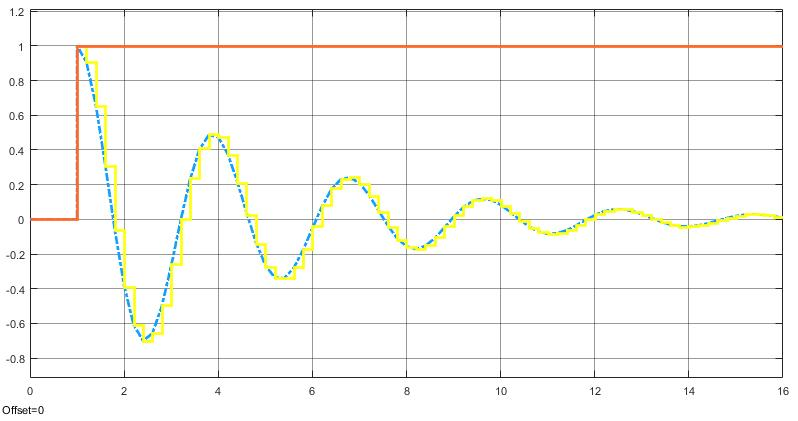
\includegraphics[width=1\linewidth]{marius/V2/Stoerungssuebertragungsfkt}
\caption{Sprungantwort der Störungsübertragungsfunktion}
\label{fig:stoerungssuebertragungsfkt}
\end{figure}
%\newpage
\section{Implementieren eines PD-Reglers und optimieren der Regelparameter nach Ziegler-Nichols}

\begin{equation}
G_{PD}(z)= \frac{K_R\left(1+\frac{T_V}{T_A}\right)z-K_R\frac{T_V}{T_A}}{z} \text{mit} K_R = 0,8K_{Krit}; T_V= 0,12T_{Krit}; T_A=0,2
\end{equation}

Für den kritischen Verstärkungsfaktors wurde $K_{Krit}= 10,353$ und $T_{Krit}=2$ festgestellt. Nach dem einsetzen ergibt das folgende Gleichung:
\begin{equation}
G_{PD}(z) = -9.93888z^{-1}+18,22128
\end{equation}
Wird die Strecke $G_S(z)$ damit geregelt ergeben sich die Führungs- und Störungssprungantworten welche in Abb. \ref{fig:fuehrungssprungantwortpd} und \ref{fig:stoerungsssprungantwortpd} zu sehen sind.\\

\begin{figure}[h!]
\centering
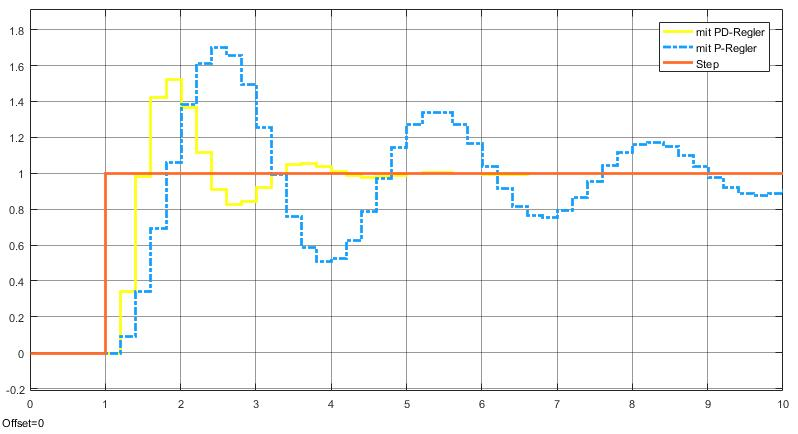
\includegraphics[width=1\linewidth]{marius/V2/Fuehrungssprungantwort_PD}
\caption{Führungssprungantwort mit PD-Regler}
\label{fig:fuehrungssprungantwortpd}
\end{figure}

\begin{figure}[h!]
\centering
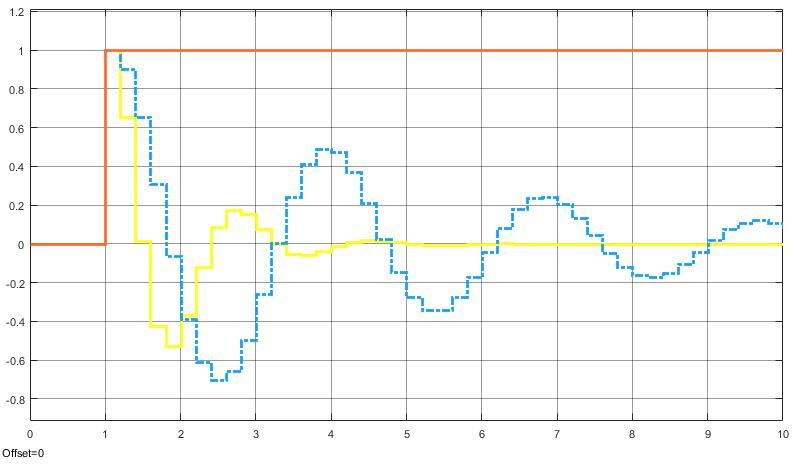
\includegraphics[width=1\linewidth]{marius/V2/Stoerungsssprungantwort_PD}
\caption{Störungssprungantwort mit PD-Regler}
\label{fig:stoerungsssprungantwortpd}
\end{figure}
%\newpage
\subsection{Interpreation der Ergebnisse}
Durch den Einsatz eines PD-Reglers statt einen reinen P-Reglers konnte sowohl das Führungsverhalten als auch das Störungsverhalten deutlich verbessert werden. Wie in den Abbildungen \ref{fig:fuehrungssprungantwortpd} und \ref{fig:stoerungsssprungantwortpd} gut zu sehen ist, konnte durch den PD-Regler und die Einstellmethode nach Ziegler Nichols, die Einschwingdauer und das Überschwingen verringt werden.


	
	
\end{document}